\documentclass[12pt,reqno]{amsart}

\usepackage{amsthm,amsmath,amssymb}
\usepackage{mathtools}
\usepackage{xcolor}
\usepackage{graphicx,wrapfig}
\usepackage[T1]{fontenc}
\usepackage{courier}
\usepackage{hyperref}
\hypersetup{
    hidelinks=true
}
\usepackage{array}
\usepackage{multirow}
\usepackage{listings}
\lstset{basicstyle=\ttfamily\footnotesize, columns=fullflexible, language=C, morekeywords={omp,task,private,pragma,parallel,reduction,single,nowait,num_threads}, numbers=left}
\newcommand{\code}[1]{\texttt{#1}}
\newcommand\MyBox[2]{
  \fbox{\lower0.75cm
    \vbox to 1.7cm{\vfil
      \hbox to 1.7cm{\hfil\parbox{1.4cm}{#1\\#2}\hfil}
      \vfil}%
  }%
}
\graphicspath{{./}}

\begin{document}

\begin{center}
\large\textbf{Assignment 3 - Report \\ COMP515 Spring 2020 - Distributed Systems} \\
\normalsize\textbf{Erhan Tezcan 0070881 \\ 30.04.2020} \\
\end{center}

\section{What is Apache Spark?}

Apache Spark is a fast, in memory data processing engine. It allows ``data workers'' to efficiently operate on distributed datasets, execute machine learning algorithms, SQL workloads or even streaming. All these operations require fast iterative access to datasets. Apache Spark comes into play here: it is very fast, with it's in-memory processing and advanced DAG execution engine. It is also a general framework. What this means is that, it's operators are general and arbitrary and this makes the whole development process easier and more flexible for a wide variety of tasks. 

\subsection{Resilient Distributed Dataset}

Apache Spark uses Resilient Distributed Dataset, abbreviated as RDD. RDD is a simple capsulation over a large dataset. From an abstract level, thinking about RDD's greatly simplified the whole deal. For example, we only have two things to do with RDDs:
\begin{itemize}
	\item \textbf{Transform}: We can transform an RDD to another RDD.
	We can for example filter some data in an RDD, or map elements of an RDD to some other RDD. We can also do basic set operations such as sampling, getting distinct values, taking union, intersection, cartesian product, or even subtracting an RDD from another RDD.
	\item \textbf{Action}: We can do an action on an RDD and get a result. This could be reduce (taking sum of all values, product of all values, etc.), counting elements, counting elements by values, taking some elements from an RDD or even taking the RDD as a collection, these are all actions that return a result rather than another RDD. The return type is a very important thing we can look at to differentiate a transform and action.
\end{itemize}

The first word in RDD is very important: Resilience. The word ``Resilience'' means the capacity to recover quickly from difficulties. Apache Spark is also resilient, thanks to the RDD characteristics. An RDD is a deterministic function of it's input. They are also immutable, and the fact of immutability solves huge problems in the world of parallel and distributed computing. RDD's are broken into multiple pieces called partitions, which are divided across clusters. If a cluster fails, Spark can recover that part of RDD thanks to resilience and immutability, and pick up where it left off. Spark does the heavy lifting for us at this point. Spark also does lazy evaluation and allows persistent memory. We won't go too much into detail of those because the assignment paper told us to not exceed 1-page for these. 

Overall, Apache Spark is a high-performance framework for distributed data processing, and this applies to domains from machine learning to basic distributed data systems. I should also include as a personal note that the developer effort is very small, the coding and usage of the framework is intuitive and clean!

\section{Bar Graph for Part-5}

In the assignment, we are asked to plot a bar graph for part 5, that shows how the computation time changes with respect to file size. The requested plot is given in figure \ref{fig:1}. We can see that the computation time is directly proportional to the file size, which was expected. However, the compute time does not always double even though the file size is doubling. This may be a benefit of the distributed system and it's parallel computation ability, as we are utilizing more than a single core.
\begin{figure}[h]
\centering
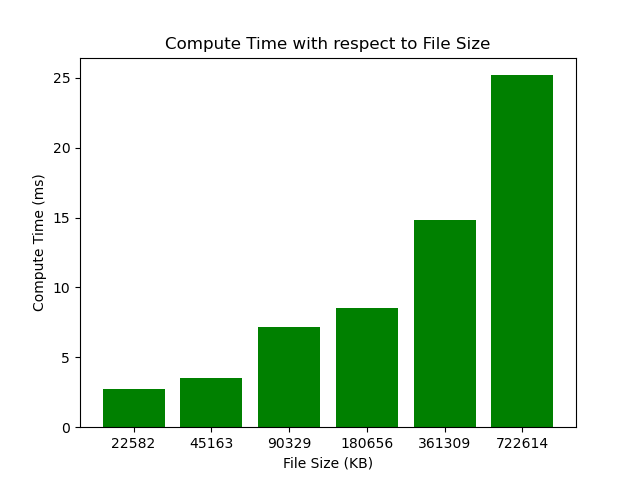
\includegraphics[width=0.9\linewidth]{plot.png}
\caption{Compute time and file size bar graph.}
\label{fig:1}
\end{figure}

\section{AWS EC2 with Spark}
I did not implement this bonus part, mainly because I am out of credits for the AWS classroom account. I spoke with our TA Waris Gill, and he will be sharing his AWS keys during the demo so that I may work on them. I believe the correct instructions are all given in this link \url{https://spark.apache.org/docs/1.6.2/ec2-scripts.html} however I did not implement them.


\end{document}